\section{SVM: Support Vector Machine}
    La $\textbf{SVM}$ è un modello di Supervised Learning che utilizza algoritmi di classificazione per problemi di classificazione tra due gruppi.
    \\[1\baselineskip]
    Rispetto agli algoritmi più recenti (come le reti neurali), presenta due vantaggi principali: maggiore velocità e migliori prestazioni con un numero piccolo di campioni.
    
    \begin{figure}[h]
        \caption{Esempio di SVM}
        \centering
        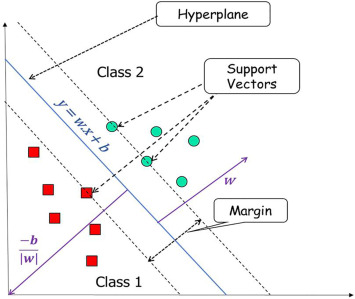
\includegraphics[width = 10cm, height = 6.7cm]{SVM-example.jpg}
    \end{figure}
    
    \clearpage

    Una SVM prende i punti del dataset e calcola l'iperpiano che separa meglio i due gruppi.
    \\
    Questa linea è la $\textbf{Decision Boundary}$ (nell'esempio sopra, tutto ciò che cade da un lato sarà classificato come rosso mentre tutto ciò che cade nell'altro sarà verde).
    \\[1\baselineskip]
    Per la SVM, il miglior iperpiano è quello che massimizza i margini dei vettori di support di ciascuna classe.
    In altre parole, trova l'iperpiano la cui distanza dell'elemento più vicino (possono essere anche più di uno se sono equamente vicini all'iperpiano) di ciascuna classe è la più grande.

    \subsection{Margini}
        Il $\textbf{margine}$ è la distanza che abbiamo tra i punti più vicini al nostro Decision Boundary, ovvero la retta.
        \\
        Esistono due tipi di margini:
        \begin{itemize}
            \item $\textbf{Hard Margin}:$ è il margine che possiamo usare quando riusciamo a separare tutti i punti da una parte e dall'altra, senza mischiarli;
            \item $\textbf{Soft Margin}:$ rilassa i vincoli dell'hard margin, permettendo che alcuni punti che dovrebbero appartenere a una classe di "sorpassare" la retta.
                Questo permette di avere meno restrizioni nel caso non esista una retta che separe bene i due cluster.
        \end{itemize}

    \subsection{Problemi di separazione non lineare}
        Immaginiamo di avere un problema del genere:

        \begin{figure}[h]
            \caption{Esempio di problema non lineare}
            \centering
            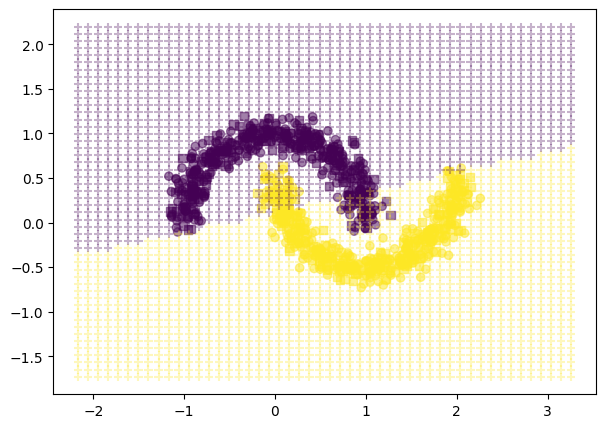
\includegraphics[width = 10cm, height = 6cm]{non-linear-problem.png}
        \end{figure}

        Per questo problema non esiste un iperpiano di due dimensioni che separa i due cluster di dati.
        \\
        La soluzione a tale problema è quella di aumentare la dimensione dello spazio su cui si sta lavorando per vedere se esiste un iperpiano che separa i due clusters.
        Dopo aver trasformato lo spazio, si può usare il regressore nel nuovo spazio creato.

        \begin{figure}[h]
            \caption{Aumento di una dimensione dello spazio}
            \centering
            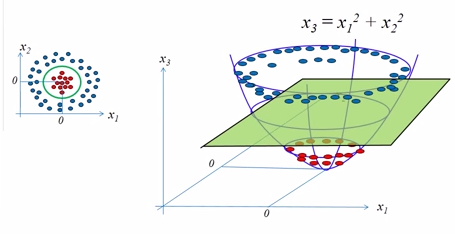
\includegraphics[width = 10cm, height = 4cm]{esempio-spazio.png}
        \end{figure}

        \begin{figure}[h]
            \caption{Risultato del regressore nel nuovo spazio}
            \centering
            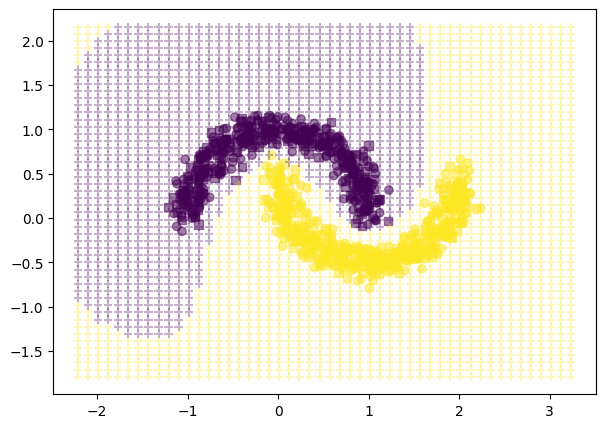
\includegraphics[width = 10cm, height = 5cm]{risoluzione-problema.png}
        \end{figure}

    \clearpage